As a natural, healthy and nutritious food, with variety of species and diverse growth environments, fish seems to be a wise choice to solve some food - related crisis regarding to the human population growth around the world. On the other hand, there is a limitation for the fish population sustainability in open seas. Global high demand, resulted in over-exploiting the oceans in the past decades (Figure \ref{fig1.1}).

\begin{figure}[H]
	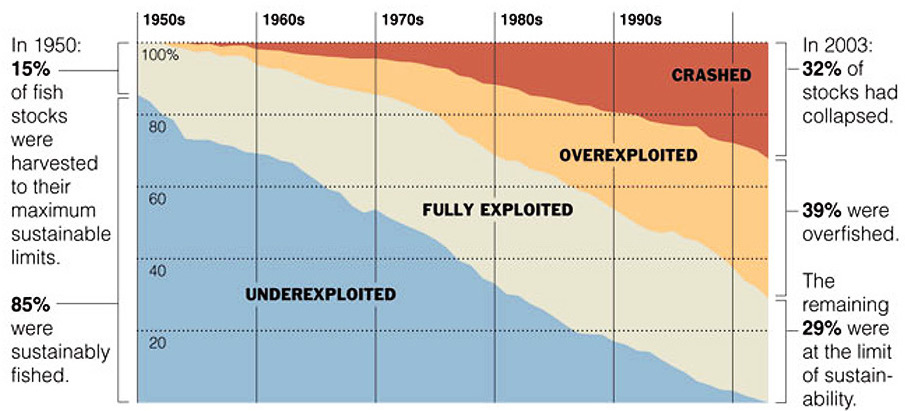
\includegraphics[width=\textwidth]{over.jpg}
	\caption{sustainable fishing between 1950 and 2003}
\end{figure}
\label{fig1.1} 

In result, some fish populations have been severely  declined during the years. Figure \ref{fig1.2} shows the population of utilized fish population between 1970 and  and 2010. As illustrated, the index for all utilized fish species indicates a 50 per cent reduction in population number globally between 1970 and 2010.

\begin{figure}[H]
	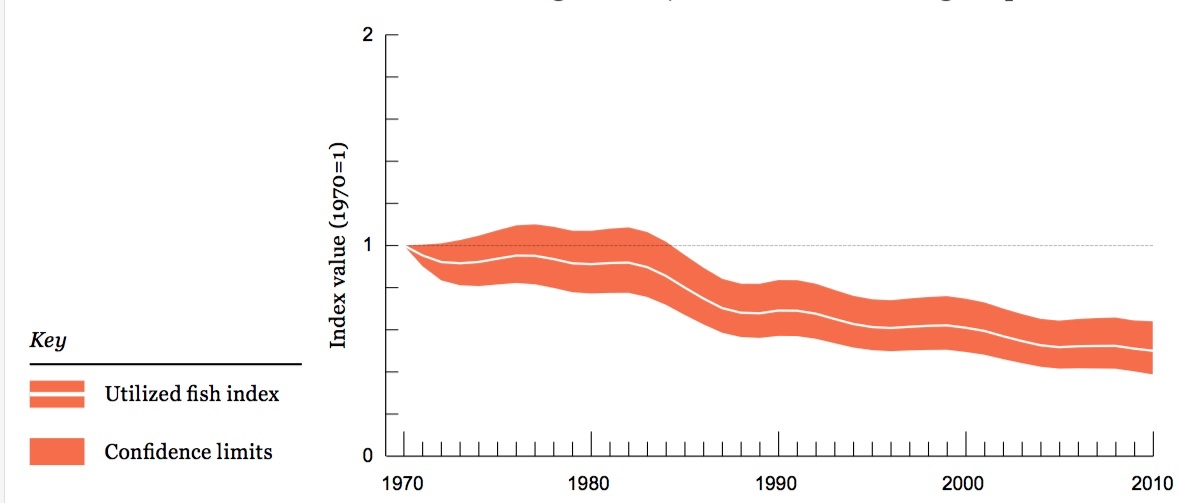
\includegraphics[width=\textwidth]{utilizedfish.jpeg}
	\caption{Utilized fish index value between 1970 and 2010}
\end{figure}
\label{fig1.2} 

One of the solutions to fish population decrease problem is to shift from fish catching to fish harvesting. This strategy can help recovering fish population and size gradually beside providing human with seafood.  Figure \ref{fig1.3} and \ref{fig1.4} shows the fish harvesting production grows in 1970 and 2010 year around the world.

\begin{figure}[H]
	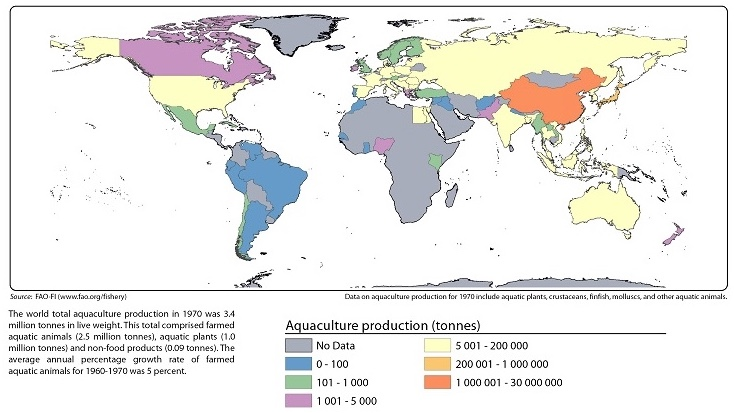
\includegraphics[width=\textwidth]{1970.jpeg}
	\caption{Aquaculture production in 1970 around the world}
\end{figure}
\label{fig1.3} 

\begin{figure}[H]
	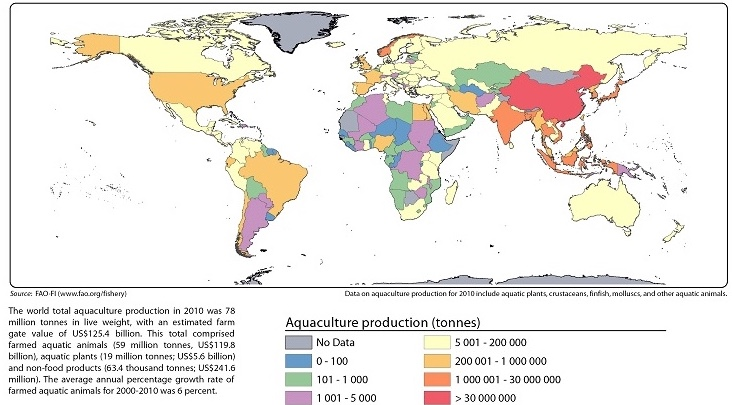
\includegraphics[width=\textwidth]{2010.jpeg}
	\caption{Aquaculture production in 2010 around the world}
\end{figure}
\label{fig1.4} 

Like any other industry, It is crucial to optimize the fish harvesting procedure to have maximum -still consistent- production in fish harvesting farms. In this work, we’re trying to describe one of the fish harvesting mathematical models and achieve the optimum fish farm population to have a consistent population.

